\subsection{Parametrisierung}
\label{sec_param}
Während der Tests ist stark aufgefallen, dass das Regressionsverfahren sehr parameterabhängig ist. Wie im vorherigen Kapitel zu sehen ist, liefert die implementierte Lösung mit der richtigen Parametrisierung ein gutes Verhalten. 
Bei falscher Parametrisierung wird die Verfolgung sehr viel schlechter bis unmöglich.\\
Große Unterschiede gibt es bei geraden und kurvigen Objekten. Als ausschlaggebende Parameter stellten sich die Gewichtungen der einzelnen Fehlerarten, die Stärke der \textit{Tikhonov Regularisierung} (siehe Gleichung \ref{F-function}) und der maximale Gesamtfehler der Regression bis zu einer \gls{transform} (siehe Abschnitt \ref{alterWorldCoords}) heraus.
Bei geraden Objekten führt eine Gleichgewichtung der Fehlerarten, eine starke \textit{Tikhonov Regularisierung} und ein hoher erlaubter Maximalfehler zu sehr guten Ergebnissen (vgl. Kapitel \ref{sec_pendel}).\\
Kurvige Objekte, wie in Abb. \ref{testSCurve} oder \ref{testStraightCirc}, führen bei einer höheren Gewichtung des Orientierungsfehlers, keiner \textit{Tikhonov Regularisierung} und einem geringeren erlaubten Maximalfehler zu guten Ergebnissen.
Problematisch ist, dass die \textit{falsche} Parametrisierung (z.B. hoher Maximalfehler für kurvige Objekte) im schlimmsten Fall zu einem großen Fehler, damit einhergehendem Sichtverlust zum Objekt und einem schlecht geschätzten Polynom führt, dass keine erneute Annäherung zum Objekt mehr gelingt. \\
Dieses Verhalten ist im Testlauf Abb. \ref{curveLost} zu beobachten. Je schärfer die Kurven und je mehr Wechsel zwischen geraden und kurvigen Bereichen im Objekt vorhanden sind, desto schwieriger ist es die richtigen Parameter zu finden. Vor allem für den Test der Geraden gefolgt von einer Kreisbahn [Abb. \ref{testStraightCirc}] war es in der Testphase schwierig die richtige Parametrisierung zu finden ohne entweder den Wechsel zwischen Kurve und Gerade (oder zurück) zu verpassen oder aber während den Geraden aufgrund des schlechten Einpendelns [Kapitel \ref{sec_pendel}] das Objekt zu verlieren.

\begin{figure}[H]
\begin{tabular}{cc}
\subfloat[Fahrtverlauf des \gls{auv}s (rot) an einer scharfen Kurve (blau) mit guten Parametern für den Objektverlauf.]{\includegraphics[height=0.4\textheight,width=0.5\textwidth]{/testlaeufe/kurvenichtverloren/auvroute.jpg}}&
\subfloat[Fahrtverlauf des \gls{auv}s (rot) an einer scharfen Kurve (blau) mit schlechteren Parametern für den Objektverlauf.]{\includegraphics[height=0.4\textheight,width=0.5\textwidth]{/testlaeufe/kurveverloren/auvroute.jpg}}\\
\subfloat[Fehler der detektierten Objektposition zur echten Objektposition.]{\includegraphics[height=0.3\textheight,width=0.5\textwidth]{/testlaeufe/kurvenichtverloren/groundTruth.jpg}}&
\subfloat[Fehler der detektierten Objektposition zur echten Objektposition.]{\includegraphics[height=0.3\textheight,width=0.5\textwidth]{/testlaeufe/kurveverloren/groundTruth.jpg}}
\end{tabular}
\caption[Testläufe am identischen Objekt mit verschiedener Parametrisierung]{Hier wurden zwei Testläufe in der identischen Umgebung (Sichtbedingungen und Objektlage) durchgeführt. Nur die Parametrisierung der Regression wurden geändert. Es ist zu beobachte, dass trotz gleich guter Detektion des Objektes (der Fehlerausschlag in \textit{c)} und \textit{d)} ist sehr ähnlich) das Objekt nur mit der richtigen Parametrisierung verfolgt werden kann.}
\label{curveLost}
\end{figure}

\subsubsection{Einpendeln}
\label{sec_pendel}
In jedem Testlauf fiel auf, dass bei erster Sicht des Objektes eine Art \texttt{Einpendeln} stattfindet, also ein zuerst großer Fehler, der dann über mehrere Meter beständig abnimmt, bis eine stabile Fahrt über dem Objekt erreicht wird. Diese Beobachtung konnte auch beim Wechsel von geraden Objektverläufen auf kurvige Verläufe gemacht werden.\\
In Abbildung \ref{figpendel} ist diese Beobachtung mit verschiedenen Parametrisierungen dargestellt.

\begin{figure}[H]
\begin{tabular}{cc}
\subfloat[Sehr gute Parametrisierung mit Gleichgewichtung der Fehlerarten, \textit{Tikhonov Regularisierung} und hohem Maximalfehler.]{\includegraphics[width=0.5\textwidth,height=0.2\textheight]{/testlaeufe/gradeGut/groundTruthPosition.jpg}}&
\subfloat[Gute Parametrisierung mit Gleichgewichtung der Fehlerarten, geringer \textit{Tikhonov Regularisierung} und weder hohem, noch geringem Maximalfehler.]{\includegraphics[width=0.5\textwidth,height=0.2\textheight]{/testlaeufe/Gradeok/groundTruthPosition.jpg}}\\
\subfloat[Schlechte Parametrisierung mit höherer Gewichtung des Orientierungsfehlers, keiner \textit{Tikhonov Regularisierung} und geringem Maximalfehler.]{\includegraphics[width=0.5\textwidth,height=0.2\textheight]{/testlaeufe/Gradeschlecht/groundTruthPosition.jpg}}
\end{tabular}
\caption[Einpendelverhalten am geraden Objekt verdeutlicht]{Testlauf mit einem geraden Objekt [Abb. \ref{testStraight}] mit unterschiedlicher Parametrisierung. Im Fehler der \gls{auv}-Position zur Objektposition ist zu erkennen, dass bei den guten Parametrisierungen der Fehler über die Zeit abfällt. Bei der sehr guten Parametrisierung (\textit{a)}) sogar noch weitaus schneller. Bei der schlechten Parametrisierung (\textit{c)}) findet keine Verringerung des Fehlers statt. Die Höhe der Ausschläge nimmt auch nicht beständig ab, wie bei den guten Parametern.}
\label{figpendel}
\end{figure}

\subsection{Systematischer Fehler}
\label{sec_sysError}
Während einiger Testläufe gab es längere Bereiche, in denen stets mit einem leichten Versatz zum Objekt gefahren wurde. Sehr deutlich zu sehen ist dieses Verhalten in den Abbildungen \ref{fig_leftCurve}, \ref{fig_rightCurve} und \ref{testSCurve}. Betrachtet man bei diesen drei Abbildungen jeweils den Fehler der detektierten Objektposition zur realen Objektposition, fällt auf, dass der Fehler um einen bestimmten Wert verteilt ist und systematisch erscheint.\\
Für das Auftreten dieses Fehlers gibt es einige mögliche Erklärungen.
Zum einen fällt auf, dass der systematische Fehler meist nach scharfen Kurven oder teilweiser Unsichtbarkeit des Objektes auftritt. Da die implementierte Lösung bei ausbleibenden Ergebnissen der Objekterkennung die Fahrthöhe erhöht, um den Sichtbereich zu vergrößern und bei erneuter Sichtung wieder auf die Zielhöhe korrigiert, wird nach einem Bereich ohne Detektion stets abwärts gefahren, was zu einem erhöhten \gls{pitch}-Wert führt.\\
Bei scharfen Kurven wird durch die Fahrteigenschaften ein höherer \gls{roll}-Wert erreicht, als bei gerader Fahrt.
Der systematische Fehler tritt also oft direkt nach Situationen auf, die eine unruhige Fahrt verursachen können. Dies lässt darauf schließen, dass die \gls{transform} von 2D- in 3D-Koordinaten (vgl. \ref{section_PicToCam})für den Fehler verantwortlich ist.\\
Eine andere mögliche Erklärung ist darin zu finden, dass das Objekt in den Bereichen mit systematischem Fehler oft leicht verdeckt ist. Verdeckte Objekte erscheinen im Binärbild schmaler. Da die Detektion im Binärbild über eine Box mit der erwarteten Breite des Objektes im Bild durchgeführt wird, führt ein schmaler erscheinendes Objekt zu Problemen. Bei optimal sichtbaren Objekten \textit{passt} diese Box am besten (die meisten Inlier), wenn der Mittelpunkt der Box in horizontaler Richtung genau in der Mitte des Objektes liegt. Bei schmaler erscheinenden Objekten \textit{passt} die Box auch an weiteren Stellen des Objekten genau so gut, wie in der Mitte. Durch den Zufallsaspekt des \gls{rans}-Algorithmus kann hier ein breiter Bereich als Objektmitte detektiert werden.\\
Gestützt wird diese Möglichkeit auch durch die Tatsache, dass die Streuung des Fehlers in Bereichen mit systematischen Fehler weitaus größer ist.
\todo{hier grafik}